\documentclass[conference]{IEEEtran}
\IEEEoverridecommandlockouts
% The preceding line is only needed to identify funding in the first footnote. If that is unneeded, please comment it out.
\usepackage{cite}
\usepackage{amsmath,amssymb,amsfonts}
\usepackage{easyReview} % 实现,高亮、删除线、替换等
\usepackage{algorithmic}
\usepackage{graphicx}
\usepackage{textcomp}
\usepackage{xcolor}
\usepackage{cuted}%%
\usepackage{subfigure}
\usepackage{booktabs}
\stripsep -3pt plus 3pt minus 2pt % 双栏公式间距
\def\BibTeX{{\rm B\kern-.05em{\sc i\kern-.025em b}\kern-.08em
    T\kern-.1667em\lower.7ex\hbox{E}\kern-.125emX}}
\begin{document}

\title{Sparse signal detection and fingerprint feature recognition based on fast 2D DFRFT
%	\\
%{\footnotesize \textsuperscript{*}Note: Sub-titles are not captured in Xplore and should not be used}
%\thanks{Identify applicable funding agency here. If none, delete this.}
}

\author{\IEEEauthorblockN{1\textsuperscript{st} Jun Yang}
\IEEEauthorblockA{\textit{ School of Mathematics and Statistics } \\
\textit{ Xidian University}\\
Xi’an, China \\
yjjdyhhxx@163.com}
\and
\IEEEauthorblockN{2\textsuperscript{nd} Jinshun Shen}
\IEEEauthorblockA{\textit{School of Mathematics and Statistics} \\
\textit{ Xidian University}\\
Xi’an, China \\
1466160996@qq.com}
%\and
%\IEEEauthorblockN{3\textsuperscript{rd} Given Name Surname}
%\IEEEauthorblockA{\textit{dept. name of organization (of Aff.)} \\
%\textit{name of organization (of Aff.)}\\
%City, Country \\
%email address or ORCID}
%\and
%\IEEEauthorblockN{4\textsuperscript{th} Given Name Surname}
%\IEEEauthorblockA{\textit{dept. name of organization (of Aff.)} \\
%\textit{name of organization (of Aff.)}\\
%City, Country \\
%email address or ORCID}
%\and
%\IEEEauthorblockN{5\textsuperscript{th} Given Name Surname}
%\IEEEauthorblockA{\textit{dept. name of organization (of Aff.)} \\
%\textit{name of organization (of Aff.)}\\
%City, Country \\
%email address or ORCID}
%\and
%\IEEEauthorblockN{6\textsuperscript{th} Given Name Surname}
%\IEEEauthorblockA{\textit{dept. name of organization (of Aff.)} \\
%\textit{name of organization (of Aff.)}\\
%City, Country \\
%email address or ORCID}
}

\maketitle

\begin{abstract}
In this paper, a two-dimensional fractional Fourier transform (2D FRFT) based fingerprint feature extraction scheme is proposed, based on the fact that the fingerprint image can be approximated as two-dimensional chirp signals. And the sparse 2D fractional Fourier transform (STDFRFT) algorithm is proposed to achieve efficient computation of 2D FRFT. The effectiveness of the proposed STDFRFT algorithm is reflected in the simulations and applications of fractional domain sparse random signal detection, convergence analysis, two-dimensional chirp signal detection and fingerprint feature recognition. 
\end{abstract}

\begin{IEEEkeywords}
fingerprint, fractional Fourier transform, chirp signals, sparse
\end{IEEEkeywords}

\section{Introduction}
 
 % 在当前信息化的社会,准确快速地识别个人身份是维护社会秩序的基本问题。然而传统的基于密码、令牌等方式的身份认证方式常会有丢失,遗忘,窃取的风险。指纹特征广泛应用于军事、民用等领域,因为独一无二的、稳定的、随身携带的、不易伪造的。一般的,指纹特征是分析指纹纹理的局部和细节结构提取出来的。然而,指纹节点特征的提取是复杂的。增强、二值化和细化处理过程计算量大。我们发现,指纹图像可以被视为二维啁啾图像的近似值。因此,我们提出了一种基于二维离散分数阶傅里叶变换(2D DFRFT)的指纹特征提取方法。还给出了二维DFRFT算法的有效实现。
 
In the current information-based society, accurate and rapid identification of individuals is a fundamental issue to maintain social order. However, traditional authentication methods (based on passwords, tokens, etc.) are often at risk of being lost, forgotten, and stolen. Fingerprint features \cite{b9} are widely used in military and civilian applications due to being unique, stable, portable and not easily forged. In general, fingerprint features are extracted by analyzing the local and detailed structure of the fingerprint texture \cite{Sun2022,Mehboob2022,Kumar2022}. However, the extraction of fingerprint node features is complex. The enhancement, binarization and refinement processes are computationally intensive. We find that the fingerprint image can be regarded as an approximation of a two-dimensional chirp image. Thus, we propose a fingerprint feature extraction method based on two-dimensional discrete fractional Fourier transform (2D DFRFT). Furthermore, an efficient implementation is also given.

% 分数阶傅里叶变换是处理非平稳信号的重要工具。它是傅里叶变换的广义形式,由于增加了一个旋转角参数,它能够联合表征时间和频率。当旋转参数从0逐渐增加,分数阶傅里叶变换能够得到信号从时域逐步变化到频域的所有特征。因此分数阶傅里叶变换可以看作信号在时频平面上的旋转。因此,指纹图像经过FRFT后能够获取更多的特征。
The fractional Fourier transform (FRFT) \cite{b6} is an important tool for dealing with nonstationary signals, especially the chirp signals. The chirp signal is strongly aggregated and even sparse in the fractional Fourier domain. As a generalized form of the Fourier transform, the FRFT can jointly characterize time and frequency due to the addition of a rotation angle parameter. The FRFT can be regarded as the rotation of the signal in the time-frequency plane. When the rotation parameter increases from zero gradually, the FRFT can obtain all the features of the signal that change from the time domain to the frequency domain gradually. Therefore, the fingerprint image can acquire more comprehensive features after FRFT.

% 将分数傅里叶变换应用于数字信号处理离不开其离散化及其高效的精确的计算。然而,这方面的研究仍不完善。目前没有任何一种离散分数阶傅里叶变换能够同时满足以下性质:酉性、旋转相加性、可退化为离散傅里叶变换、逼近连续分数阶傅里叶变换、可写成闭合形式、计算复杂度低。采样型离散分数阶傅里叶变换是最直观的离散化定义,它是由连续的分数阶傅里叶变换核直接采样得到的。当不要求旋转相加性时,采样型离散分数阶傅里叶变换被广泛应用在各个领域。这篇文章中我们考虑引用最多的Pei型DFRFT.
The application of FRFT to digital signal processing is inseparable from its discretization and efficient and accurate calculation \cite{b4}. However, research in this area is still incomplete. At present, there is no discrete fractional Fourier transform (DFRFT) that can satisfy all the following properties: unitary, rotational additivity, degenerate to discrete Fourier transform, approximate continuous FRFT, can be written in closed form, calculation low complexity. Sampling DFRFT is the most intuitive definition of discretization, which is directly sampled by a continuous FRFT kernel. If rotational additivity is not required, the sampled DFRFT is widely used in various fields. We consider the most cited Pei-type \cite{b2} DFRFT in this paper.

% 一般的,二维离散分数阶傅里叶变换的计算通过转化为一维实现。具体的,首先对二维信号的各行(列)进行1D DFRFT, 然后对得到的信号的各列(行)计算1D DFRFT.计算复杂度高,不能满足大数据和实时处理的需要。启发于全新的估计2D DFT算法MARS-SFT的思路,我们将进一步优化2D DFRFT的计算结构。
In general, the computation of the 2D DFRFT \cite{Kumari2021} is accomplished by converting to 1D DFRFT. Specifically, 1D DFRFT is first performed on each row (column) of the two-dimensional signal, and then 1D DFRFT is calculated on each column (row) of the obtained signal. The Pei-type DFRFT requires two chirp products and one FFT operation. Therefore, a 2D DFRFT \eqref{2D DFRFT} of $s({t_1},{t_2})$ needs $2({N_1} + {N_2})$ chirp products and ${N_1} + {N_2}$ FFT operations, where the size of $s({t_1},{t_2})$ is $(N_1,N_2)$. For applications with large amounts of data, this calculation is very expensive. It also cannot meet the needs of real-time processing. Inspired by the idea of MARS-SFT \cite{b1} algorithm to estimate 2D DFT, we will propose the Sparse Two-Dimensional Fractional Fourier Transform (STDFRFT) algorithm to further optimize the computational structure of 2D DFRFT. This wil lead to fast and effective fingerprint feature recognition.


\section{Two-Dimensional Discrete Fractional Fourier Transform}

In this section, we will describe the definition of 2D DFRFT and give its closeable variants. 

The 2D DFRFT of the signal $s({t_1}, {t_2})$ with order $(\alpha,\beta)$ is defined as
\begin{align}
     O_s^{\alpha ,\beta }({u_1},{u_2}) = \sum\limits_{{t_1} = 0}^{{N_1} - 1} {\sum\limits_{{t_2} = 0}^{{N_2} - 1} {[{K_\alpha }({u_1},{t_1}) \otimes {K_\beta }({u_2},{t_2})]} } s({t_1},{t_2})
\end{align} 
where ${t_1},{u_1} = 0,1, \cdots, N_1-1$, and ${t_2},{u_2} = 0,1, \cdots, N_2-1$. And $N_1,N_2$ are integers. Meanwhile, $\otimes $ represents the tensor product and ${K_\lambda}$ denotes the 1D fractional Fourier transform kernel with order $\lambda $.

According to the definition of Pei-type DFRFT, the $O_s^{\alpha ,\beta }({u_1},{u_2})$ can be rewritten as:
\begin{align} \label{2D DFRFT}
      &O_s^{\alpha ,\beta }({u_1},{u_2}) = \notag \\
      &\left\{ {\begin{array}{*{20}{c}}
      		{A{E_u}\sum\limits_{{t_1} = 0}^{{N_1} - 1} {\sum\limits_{{t_2} = 0}^{{N_2} - 1} {s({t_1},{t_2})} } {E_t}{E_{ut}}}&{\sin \alpha ,\sin \beta  > 0}\\
      		{A{E_u}\sum\limits_{{t_1} = 0}^{{N_1} - 1} {\sum\limits_{{t_2} = 0}^{{N_2} - 1} {s({t_1},{t_2})} } {E_t}E_{ut}^{ - 1}}&{\sin \alpha ,\sin \beta  < 0}
      \end{array}} \right.
\end{align}
where 
\begin{align}
	A =  \sqrt {\frac{{(\sin \alpha  - j\cos \alpha )(\sin \beta  - j\cos \beta )}}{{{N_1}{N_2}}}}\\
	{E_u} =  \exp \left\{ j\frac{{u_1^2\Delta u_1^2}}{{2\tan \alpha }} + j\frac{{u_2^2\Delta u_2^2}}{{2\tan \beta }}\right \}\\
	{E_t} =  \exp  \left\{ j\frac{{t_1^2\Delta t_1^2}}{{2\tan \alpha }} + j\frac{{t_2^2\Delta t_2^2}}{{2\tan \beta }}\right\} \\
	{E_{ut}} =  \exp\left \{  - j2\pi (\frac{{{t_1}{u_1}}}{{{N_1}}} + \frac{{{t_2}{u_2}}}{{{N_2}}})\right\} 
\end{align}
and $\Delta {t_1},\Delta {t_2}$, $\Delta {u_1},\Delta {u_2}$ denote the sampling intervals on time and  fractional Fourier domain, respectively. They must satisfy the following constraints:
\begin{align} 
	\Delta {t_1}\Delta {u_1} = \frac{{2\pi \left| {\sin \alpha } \right|}}{{{N_1}}} \\
	\Delta {t_2}\Delta {u_2} = \frac{{2\pi \left| {\sin \beta } \right|}}{{{N_2}}}
\end{align}
%Specially, if $ \alpha=\beta=2c\pi $, the 2D DFRFT degenerates into identity transform (no transform). If $ \alpha=\beta=(2c+1)\pi $ the 2D DFRFT performs symmetric transform. $ c$ is any integer and these are easy to achived. If $ \alpha=\beta= (2c+1/2)\pi $, 2D DFRFT degenerates into traditional 2D discrete Fourier transform (DFT). If $ \alpha=\beta= (2c+3/2)pi $, the 2D DFRFT performs the traditional 2D inverse discrete Fourier transform (IDFT). If $ \alpha= (2c_1+1/2)\pi, \beta=2c_2\pi$, 2D DFRFT  degenerates into only row DFT transforms. If $ \alpha= 2c_1\pi, \beta=(2c_2+1/2)\pi$, 2D DFRFT  degenerates into only column DFT transforms. $ c,c_1,c_2$ are any integer and these can be calculated by FFT. In particular, if the frequency domain is sparse, SFT can be used.
It can be found that \eqref{2D DFRFT} is simplified to 2D DFT if $ \alpha=\beta= (2c+1/2)\pi $. And if $ \alpha=\beta= (2c+3/2)pi $, the 2D DFRFT degenerates into 2D inverse Fourier transform. Where $c$ is arbitrary integer. 


\section{Sparse Two-Dimensional Fractional Fourier Transform}\label{AA}
%二维分数阶傅里叶变换通常通过对二维信号的所有行进行一维分数阶傅里叶变换然后对所得信号的所有列进行一维分数阶傅里叶变换得到。
In this section, we will introduce the proposed sparse 2D fractional Fourier transform (STDFRFT) algorithm. Generally, a two-dimensional(2D) FRFT is obtained by applying a one-dimensional FRFT to all rows of a two-dimensional signal and then applying a one-dimensional FRFT to all columns of the resulting signal. Differently, the proposed STDFRFT method uses a new structure to greatly reduce the computational complexity.

% 信号s的2D DFRFT中除了k个位置外其余全部是可忽略的。 我们算法的目标是估计k个重要频率的幅度和位置。
Suppose the 2D DFRFT $O_s^{\alpha ,\beta }({u_1},{u_2})$ of the $(N_1,N_2)$-point signal $s({t_1}, {t_2})$ satisfies that all but $k$ coefficients are negligible. Where $k$ is an integer much smaller than $N = {N_1}{N_2}$. That is, the signal $s({t_1}, {t_2})$ is $k$-sparse, and the sparsity is $k$. The goal of our STDFRFT algorithm is to estimate the locations $(\xi _1^i,\xi _2^i)_{i = 1}^k$ and amplitudes $[O_s^{\alpha ,\beta }(\xi _1^i,\xi _2^i)]_{i = 1}^k$ of the $k$ significant frequencies. Without loss of generality, we suppose $\sin \alpha  > 0,\sin \beta  > 0$ and the structure of STDFRFT algorithm is as follows.

%为了弥补载波中chirp基的影响,我们将原始信号与chirp信号相乘,构造一个二维稀疏傅里叶变换(2D SFT)阶段的输入信号.
\paragraph{First chirp modulation} To compensate for the effect of the chirp basis, we multiply the original signal $s({t_1}, {t_2})$ with a chirp signal and construct an input signal of two-dimensional sparse Fourier transform (2D SFT) stage.
\begin{align}
	{c}({t_1},{t_2}) = s({t_1},{t_2})\exp \left\{ {j\frac{{t_1^2\Delta t_1^2}}{{2\tan \alpha }} + j\frac{{t_2^2\Delta t_2^2}}{{2\tan \beta }}} \right\}{\rm{ }}
\end{align}
where ${t_1} = 0,1, \cdots {N_1} - 1$ and ${t_2} = 0,1, \cdots {N_2} - 1$. Meanwhile, $\Delta {t_1},\Delta {t_2}$ denote the sampling intervals on time domain. And $\alpha ,\beta$ are the orders of the two dimensions, respectively.

% 我们使用迭代算法来估计c的频谱。每次迭代使用混叠滤波器分桶,然后,使用简单的运算将B点FFT得到的一维频谱映射到估计频谱最佳逼近。
\paragraph{Two-dimensional sparse Fourier transform} We use an iterative algorithm to estimate the spectrum of ${c}({t_1},{t_2})$. In each iteration, the aliasing filter is used to divide the $N$ frequencies into $B = LCM({N_1},{N_2})$ parts, called buckets. It is worth noting that the spectrum $F_c^r({u_1},{u_2})$ to be estimated in the $r$-th iteration is obtained by subtracting the result estimated by previous iterations from the original spectrum ${F_c}({u_1},{u_2})$. Then, a simple operation is used to map the 1D spectrum obtained by the $B$-point FFT to the approximation of ${F_c^r}({u_1},{u_2})$.

%我们在c中提取相互平行的三个切片,分别进行fft运算后即可得到三组桶。
The analysis of the bucketing process is as follows. We extract slices ${b_0}(l),{b_1}(l),{b_2}(l)$ in ${c}({t_1},{t_2})$ that are parallel to each other:
\begin{align}
	{b_0}(l) &= c({[{\alpha _1}l + {\tau _1}]_{{N_1}}},{[{\alpha _2}l + {\tau _2}]_{{N_2}}})\\
	{b_1}(l) &= c({[{\alpha _1}l + {\tau _1} + 1]_{{N_1}}},{[{\alpha _2}l + {\tau _2}]_{{N_2}}})\\
	{b_2}(l) &= c({[{\alpha _1}l + {\tau _1}]_{{N_1}}},{[{\alpha _2}l + {\tau _2} + 1]_{{N_2}}})
\end{align}
where $l = 0,1, \cdots B - 1$, and ${\alpha _1}, {\alpha _2},{\tau _1},{\tau _2}$ are arbitrary integrals with ${\alpha _1},{\tau _1} \in [0,{N_1} - 1]$, and $ {\alpha _2},{\tau _2} \in [0,{N_2} - 1] $. It is must satisfied that $({\alpha _1},{\alpha _2}),({\alpha _1},{B \mathord{\left/
		{\vphantom {B {{N_2}}}} \right.
		\kern-\nulldelimiterspace} {{N_2}}}),({\alpha _2},{B \mathord{\left/
		{\vphantom {B {{N_1}}}} \right.
		\kern-\nulldelimiterspace} {{N_1}}})$ are coprime pairs. And ${[a]_b}$ denotes $a$ mod $b$.

Three groups of buckets can be obtained after performing the FFT operation on slices ${b_0}(l),{b_1}(l),{b_2}(l)$, respectively. 
\begin{align}
	{F_{{b_0}}}(h) &= \frac{B}{N}\sum\limits_{({u_1},{u_2})} {{F_c}({u_1},{u_2})\exp (j2\pi [\frac{{{u_1}{\tau _1}}}{{{N_1}}} + \frac{{{u_2}{\tau _2}}}{{{N_2}}}])} \Theta \\
	{F_{{b_1}}}(h) &= \frac{B}{N}\sum\limits_{({u_1},{u_2})} {{F_c}({u_1},{u_2})\exp (j2\pi [\frac{{{u_1}{\tau _1} + {u_1}}}{{{N_1}}} + \frac{{{u_2}{\tau _2}}}{{{N_2}}}])} \Theta \\
	{F_{{b_2}}}(h) &= \frac{B}{N}\sum\limits_{({u_1},{u_2})} {{F_c}({u_1},{u_2})\exp (j2\pi [\frac{{{u_1}{\tau _1}}}{{{N_1}}} + \frac{{{u_2}{\tau _2} + {u_2}}}{{{N_2}}}])} \Theta
\end{align}
where $h = 0,1, \cdots B - 1$ and $N = {N_1}{N_2}$. Moreover, ${F_c}({u_1},{u_2})$ is the 2D DFT of ${c}({t_1},{t_2})$ on $({u_1},{u_2})$. $\Theta $ is an impulse function with
\begin{align} \label{impulse}
	 \Theta  = \delta (\frac{{{u_1}{\alpha _1}}}{{{N_1}}} + \frac{{{u_2}{\alpha _2}}}{{{N_2}}} - \frac{h}{B})
\end{align}
%根据上述公式,第h桶的值是N/B个频率的投影和。 反过来,()处的频率分到桶h.因此,所有的频率被均匀地、正交地分到B个桶中。
According to \eqref{impulse}, the value of the $h$-th bucket is equal to the sum of the projection of $N/B$ frequencies $(u_1,u_2)$ which satisfy $\frac{{{u_1}{\alpha _1}}}{{{N_1}}} + \frac{{{u_2}{\alpha _2}}}{{{N_2}}} - \frac{h}{B} = 0$. Conversely, the frequency at $(u_1,u_2 )$ is divided into bucket $h$ with
\begin{align}
	h = {\left[\frac{{B{u_1}{\alpha _1}}}{{{N_1}}} + \frac{{B{u_2}{\alpha _2}}}{{{N_2}}}\right]_B} 
\end{align}
Therefore, all frequencies are divided into $B$ buckets evenly and orthogonally.

% 频率估计过程的分析如下。为了方便,减去之前迭代影响后的桶值仍记为...重要频率一定被分到大值桶中。
The analysis of the frequency estimation process is as follows. For convenience, the buckets' values after subtracting the influence of the previous iteration is still recorded as $	{F_{{b_0}}}(h),	{F_{{b_1}}}(h),	{F_{{b_2}}}(h)$. Because the signal $s({t_1}, {t_2})$ is $k$-sparse, the spectrum to be estimated is sparse. Therefore, some buckets only include negligible noises and significant frequencies must be divided into largest-value buckets. Assuming that the large-value bucket $h$ contains only one significant frequency, the location $({\xi _1},{\xi _2})$ and amplitude ${F_c^r}({\xi _1},{\xi _2})$ of this frequency can be estimated as:
\begin{align} \label{est1}
	{\xi _1} &= {\left[\frac{{{N_1}}}{{2\pi }}\phi (\frac{{{F_{{b_1}}}(h)}}{{{F_{{b_0}}}(h)}})\right]_{{N_1}}}\\ \label{est2}
	{\xi _2} &= {\left[\frac{{{N_2}}}{{2\pi }}\phi (\frac{{{F_{{b_2}}}(h)}}{{{F_{{b_0}}}(h)}})\right]_{{N_2}}}\\
	F_c^r({\xi _1},{\xi _2}) &= N{F_{{b_0}}}(h)\exp \left[ - j2\pi (\frac{{{\xi_1}{\tau _1}}}{{{N_1}}} + \frac{{{\xi_2}{\tau _2}}}{{{N_2}}})\right]/B
\end{align}
where $\phi (a)$ denotes the phase of $a$ and ${[a]_b}$ denotes $a$ mod $b$.

%对于无噪声的信号,每次迭代经过上述分桶和估计过程即可很大概率的精确估计大部分重要频率。 对于含躁信号,18,19解码的位置是非整数,我们需要将其四舍五入。不幸的是,这可能引起解码误差。为了降低解码错误的概率,我们采用投票法。具体的,每次迭代中执行q次内循环,并记录解码的位置。如果位置被标记超过p次,我们认为它就是重要频率的位置。经过几次迭代以后,没有被解码的频率设置振幅为0。此外,如果频率被重复解码,振幅取和。
For a noise-free signal, after the above bucketing and estimation process in each iteration, most of the significant frequencies can be estimated accurately with a high probability. For a noisy signal, the positions decoded by \eqref{est1}, \eqref{est2} are nonintegers and we need to round them up. Unfortunately, this may lead to decoding errors. To reduce the probability of decoding errors, the voting method is utilized. Specifically, the inner loop is executed $q$ times in each iteration, and the decoded positions are recorded. If a location is marked more than $p$ times, we consider it to be the location of a significant frequency. After several times iterations, amplitude of the frequencies that are not decoded are set to zero. In addition, if frequencies are decoded repeatedly, the amplitudes are summed.


%为了由傅里叶域调制到分数阶傅里叶域,我们将得到的估计结果乘以另一个chirp函数,得到STWFRFT的最终结果。
\paragraph{Second chirp modulation} 
To modulate from the Fourier domain to the fractional Fourier domain, we multiply the above estimation by another chirp signal and get the final result of STDFRFT:
\begin{align}
		{\tilde O}_s^{\alpha ,\beta }({u_1},{u_2}) = A{F_c}({u_1},{u_2})\exp \left\{ {j\frac{{u_1^2\Delta u_1^2}}{{2\tan \alpha }} + j\frac{{u_2^2\Delta u_2^2}}{{2\tan \beta }}} \right\}		
\end{align}
where ${u_1} = 0,1, \cdots {N_1} - 1$ and ${u_2} = 0,1, \cdots {N_2} - 1$. Meanwhile, $\Delta {u_1},\Delta {u_2}$ denote the sampling intervals on fractional Fourier domain. And $\alpha ,\beta$ are the orders of the two dimensions, $A$ is constant with
\begin{align}
	A = \sqrt {\frac{{(\sin \alpha  - j\cos \alpha )(\sin \beta  - j\cos \beta )}}{{{N_1}{N_2}}}} 
\end{align}
 
\section{Numerical Simulation and Applications} 
 
\subsection{Fractional Domain Sparse Random Signal Detection} 

%为了检验算法的有效性,我们构造分数域稀疏的随机信号。具体的, 我们算法检测的结果 我们设置信号的稀疏度为5,并且5个重要频率的位置和振幅是随机的。 分解为1D的检测结果 噪声下的结果  比较(时间、误差、样本)
In order to verify the effectiveness of the algorithm, we will construct a random signal with sparse fractional domain. Specifically, we set the sparsity of the signal to $5$ in the fractional Fourier domain with orders $(1.2566^{\circ},1.2566^{\circ})$. The positions and amplitudes of the five significant frequencies are random. At the same time, additive white Gaussian noise with SNR=$26.9825dB$ is added. The constructed signal with a size of (256,256) is shown in Fig. \ref{random}. 

First, we detect the signal by decomposing 2D DFRFT to two groups of 1D DFRFT, which is implemented by direct method. And Fig. \ref{Decomp_random} shows the results of random sparse signal detection. Then, signal detection in the fractional Fourier domain is performed by the proposed STDFRFT algorithm. The program has one iteration in total. We set three loops in each iteration, and the voting threshold is 2. The obtained results are shown in Fig. \ref{Our_random}. In order to show more clearly, we give the corresponding top views in Fig. \ref{Decomp_fu} and Fig. \ref{Our_fu}, respectively. As can be seen from Fig. \ref{det_sparse}, our algorithm accurately detects all the significant components in the noisy situation. Finally, to visualize algorithm performance, we measured the computation time and the number of samples used in the time domain for both obove methods and methods in \cite{Ozaktas,b2,JR}. Meanwhile, the ${L_2}$ errors between the decoded results and the original fractional domain spectrum (no noise) are also computed. The table \ref{compare} presents the time, ${L_2}$ error and the samples number for the two methods clearly. And our method is optimal in every respect. 
 

 \begin{table}[t]
	\caption{Comparison of the methods}
	\begin{center}
		\begin{tabular}{cccc}
			\toprule %第一根线
			& \textbf{\textit{Time/s}}& \textbf{\textit{${L_2}$ error}}& \textbf{\textit{samples number}} \\
			\midrule %中间的线
			{Direct method}& {13.3246} & {31.5184} & {65536} \\
			{Decomposing and \cite{Ozaktas} method}&  {0.25001} & {42.1781} & {65536} \\
			{Decomposing and \cite{b2} method}& {0.01396} & {31.7074} &{65536} \\
			{Decomposing and \cite{JR} method}& { 0.45293} & {25.4828} &{65536} \\
			Our result& 0.00630 & 6.9803 & 2304 \\
			\bottomrule %最后一根线
		\end{tabular}
		\label{compare}
	\end{center}
\end{table}

\begin{figure}[t]
	\centerline{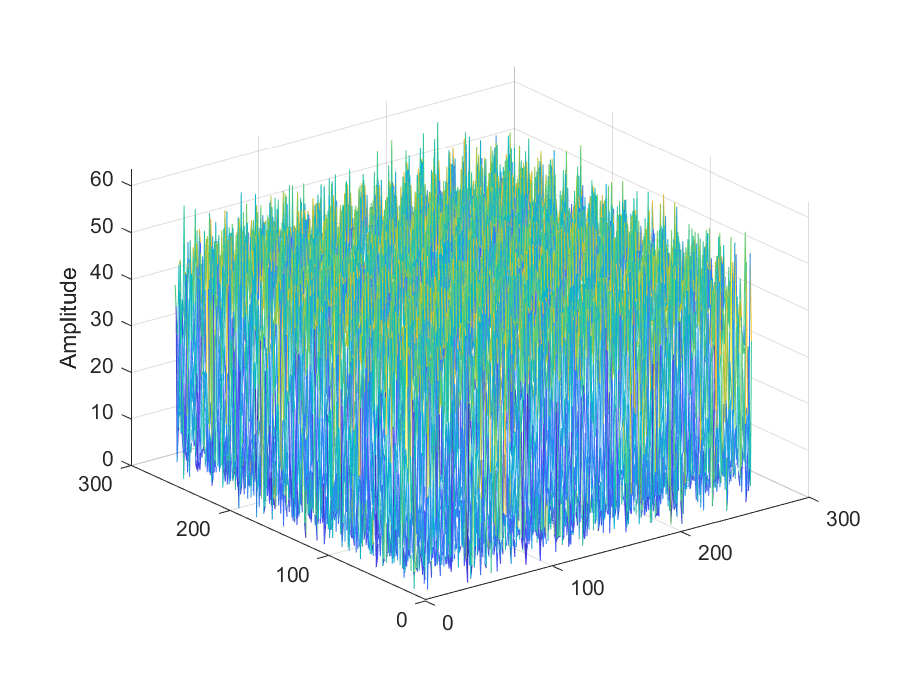
\includegraphics[width=55 mm]{fig/random_time.eps}}
	\caption{The experimental signal.}
	\label{random}
\end{figure}
\begin{figure}[t]
	\centering
	\subfigure[Result by decomposing.] 	{%第一张子图
		\begin{minipage}[]{42 mm} 				
			\centerline{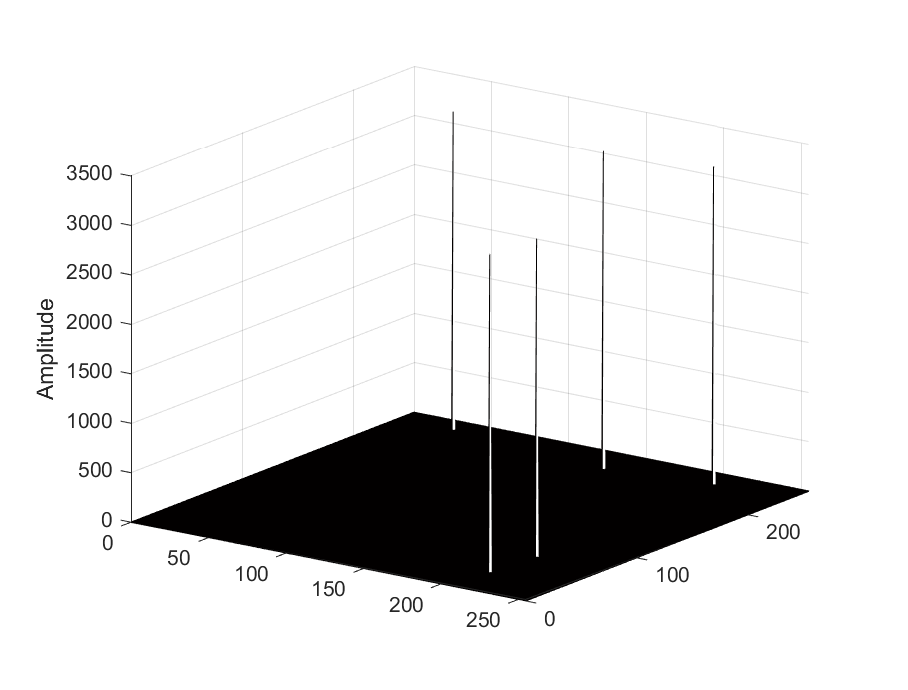
\includegraphics[width=50 mm]{fig/Decomp_random.eps}}
		\end{minipage}
		\label{Decomp_random}	}
	\subfigure[Our result.] {%第2张子图
		\begin{minipage}[]{42 mm} 				
			\centerline{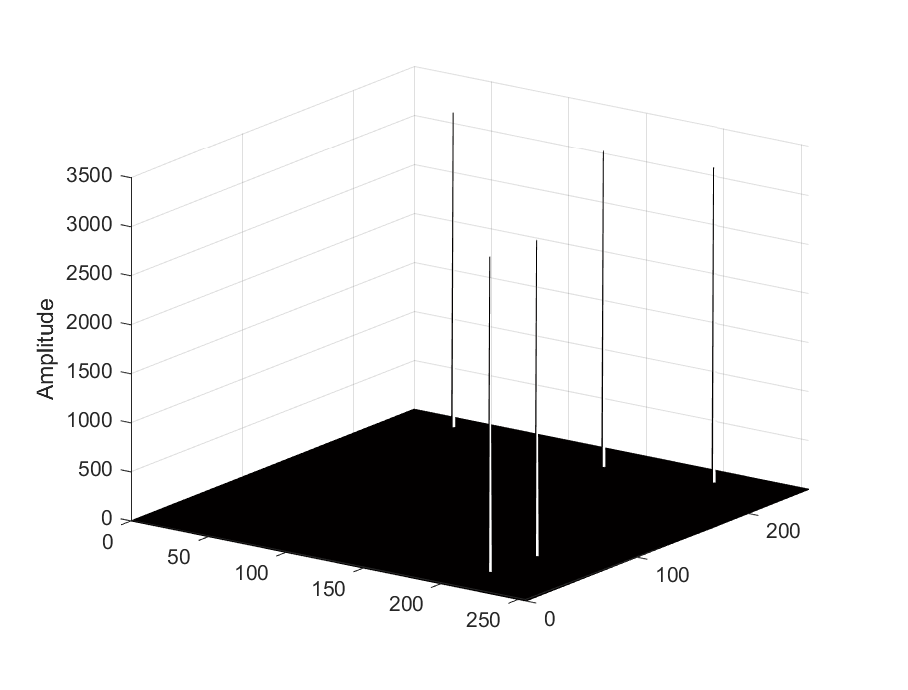
\includegraphics[width=50 mm]{fig/Our_random.eps}}
		\end{minipage}
		\label{Our_random}	}
	
	\subfigure[Result by decomposing.] 	{%第一张子图
		\begin{minipage}[]{42 mm} 				
			\centerline{\includegraphics[width=50 mm]{fig/Decomp_fu.eps}}
		\end{minipage}
		\label{Decomp_fu}	}
	\subfigure[Our result.] {%第2张子图
		\begin{minipage}[]{42 mm} 				
			\centerline{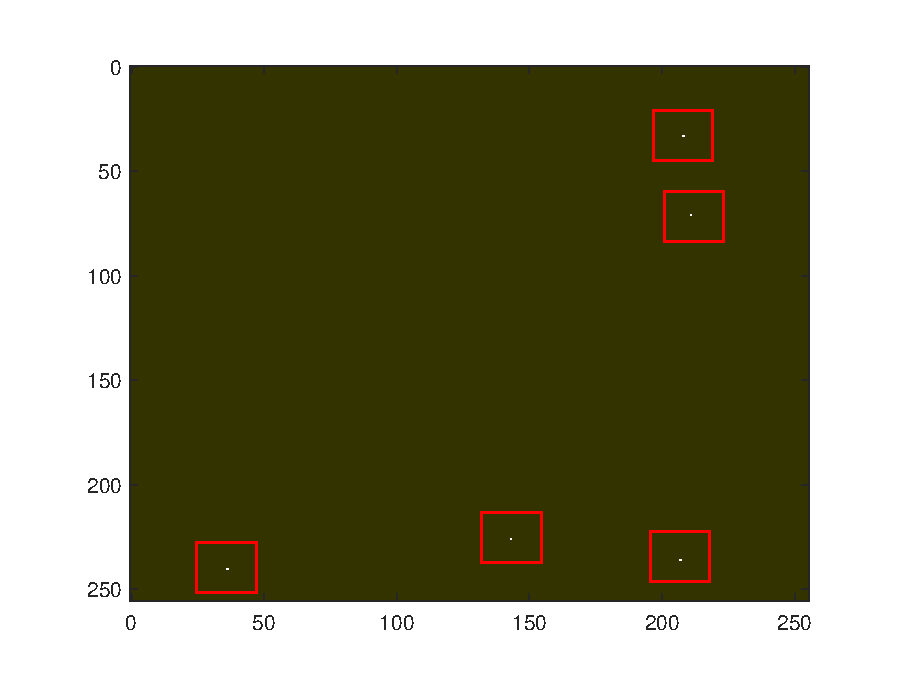
\includegraphics[width=50 mm]{fig/Our_fu.eps}}
		\end{minipage}
		\label{Our_fu}	}
	\caption{Detection Results of Sparse Random Signals in Fractional Domain.}  %大图名称	
	\label{det_sparse}
\end{figure}

\subsection{{Convergence of the STDFRFT algorithm}} 
% 在这一节验证算法的收敛性。具体的,讨论算法最小的迭代次数,使得所有的频率被正确检测。分数域稀疏随机信号仍然被考虑,信号的稀疏度k取为[100--600],信号大小N=N1*N2为65536,其中分别令(N1,N2)等于(256,256),(512,128),(1024,64). 此外,信号被添加了SNR=34.1541的复高斯白噪声。图converge展示了仿真的结果。不难得到,STDFRFT算法是收敛的,且迭代次数随着稀疏度的增加而增加。
{In this subsection, we are going to verify the convergence of the STDFRFT algorithm. Specifically, we will discuss the minimum number of iterations of the STDFRFT algorithm to detect all significant frequencies successfully. The fractional domain sparse random signals are still considered. And the sparsity $k$ of the signals are taken to be $k \in [100,200,300,400,500,600]$. The signal size $N=N_1N_2$ is 65536, where $(N1,N2)$ is equal to (256,256), (512,128), and (1024,64) respectively. In addition, the signals are added with complex Gaussian white noise with SNR = 34.1541dB. Fig. \ref{converge} shows the results of the simulation. It is not difficult to obtain that the STDFRFT algorithm is convergent. Moreover, the number of iterations increases with the increase of sparsity and $B=LCM(N_1,N_2)$.}

\begin{figure}[t]
	\centerline{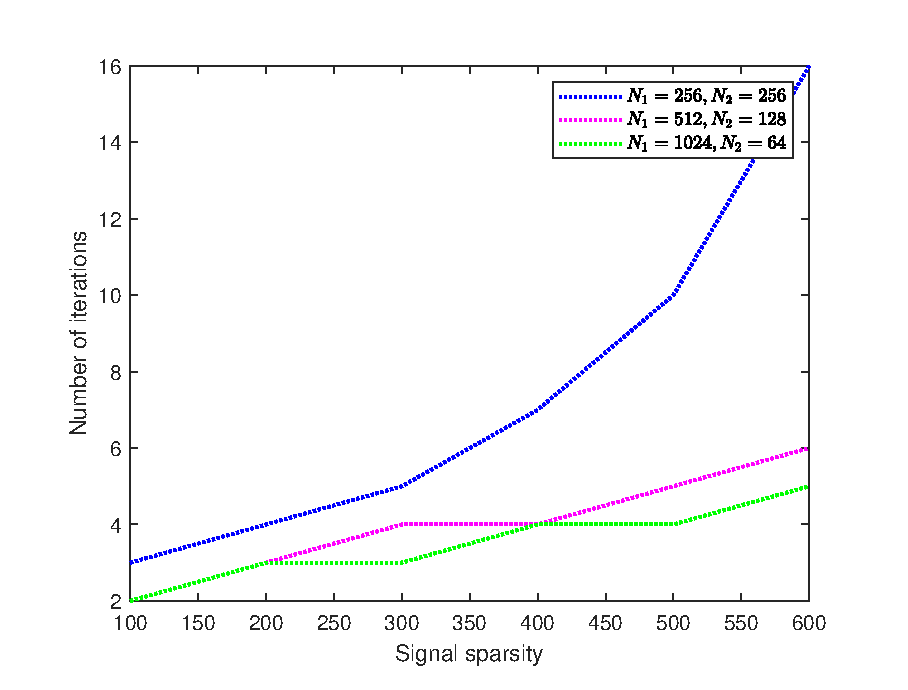
\includegraphics[width=65 mm]{fig/converge.eps}}
	\caption{{Number of iterations of STDFRFT algorithm vs. sparsity of signal.}}
	\label{converge}
\end{figure}

\subsection{Two-dimensional chirp signal detection}
 %线性调频信号在脉冲压缩、雷达载波、声纳等方面已经受到了广泛的研究和应用。二维线性调频信号同样也是非常重要的非平稳信号之一。 根据定义,分数阶傅里叶变换能够将信号用chirp正交基分解。因此FRFT对于处理线性调频信号具有天然的优势,并且具有很强的能量聚集性。用于实验的chirp信号如图所示。 为了校验仿真结果,我们记录了发射脉冲的雷达参数。具体的,脉冲幅度等于3。调频率和中心频率分别为(-16.4Hz/s,-7.8Hz/s) (640Hz,896Hz).
 In this subsection, we will apply the proposed STDFRFT algorithm to detect two-dimensional chirp signals. The chirp signal has been studied and applied in pulse compression, radar carrier, sonar and so on widely. The two-dimensional chirp signal is also one of the important nonstationary signals. By definition, the FRFT can decompose a signal with a chirp orthonormal basis. Therefore, FRFT has a natural advantage for processing chirp signals, and has strong energy concentration. Meanwhile, the fractional Fourier domain of the chirp signal is sparse at the optimal rotation angle. The chirp signal used for the experiment is shown in the Fig. \ref{chirp}. The sampling rate at discretization is 4096 Hz/s, and the pulse duration is $2^{-6}$ seconds. To check the simulation results, we recorded the radar parameters of the transmitted pulses. Specifically, the pulse amplitude is equal to 3. The modulation frequency and center frequency are (-16.4Hz/s, -7.8Hz/s) and (640Hz, 896Hz), respectively.

 First, we use a discrete polynomial phase transform to estimate the frequency modulation in both dimensions of the signal. Then, the optimal rotation angle of the chirp signal is estimated using the frequency modulation. Finally, the STDFRFT algorithm is used to estimate the fractional Fourier spectrum of the chirp signal. The program has one iteration in total. We set three loops in each iteration, and the voting threshold is 2. Fig.\ref{chirp_our} shows the estimated result and its top view. It is easy to get that the location of the dominant frequency is the center frequency of the chirp signal. The amplitude estimated by the algorithm is 2.999998, which is close to the true amplitude of the signal. Therefore, the detection of the 2D chirp signal is well done.

  \begin{figure}[t]
	\centering
	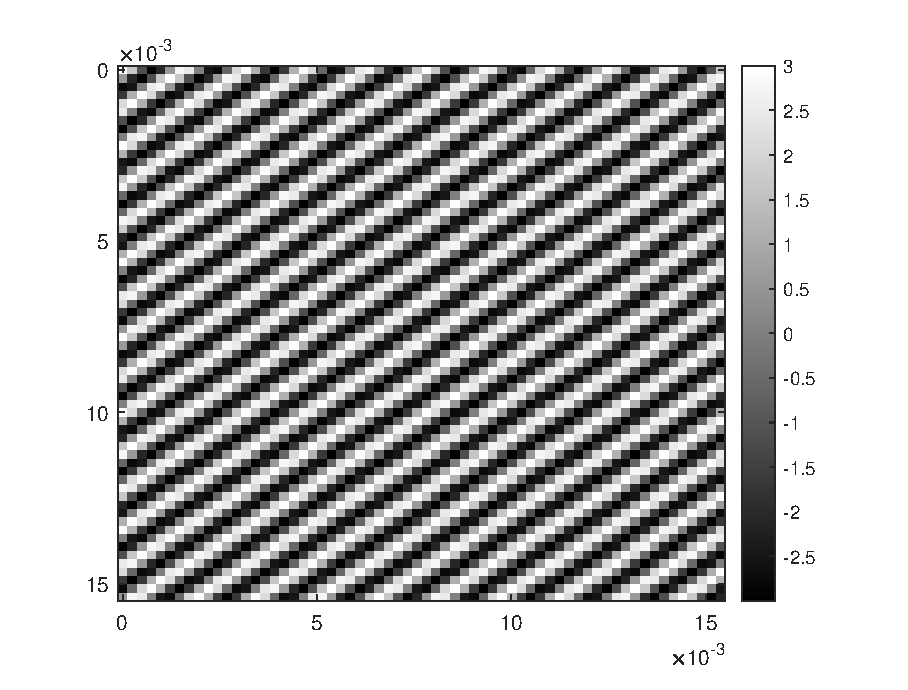
\includegraphics[width = 55 mm]{fig/chirp.eps}
	\caption{Two-dimensional chirp signal}
	\label{chirp} 
\end{figure}
\begin{figure}[t]
	\centering
	\subfigure[Amplitude spectrum in fractional Fourier domain.] 	{%第一张子图
		\begin{minipage}[]{45 mm} 				
			\centerline{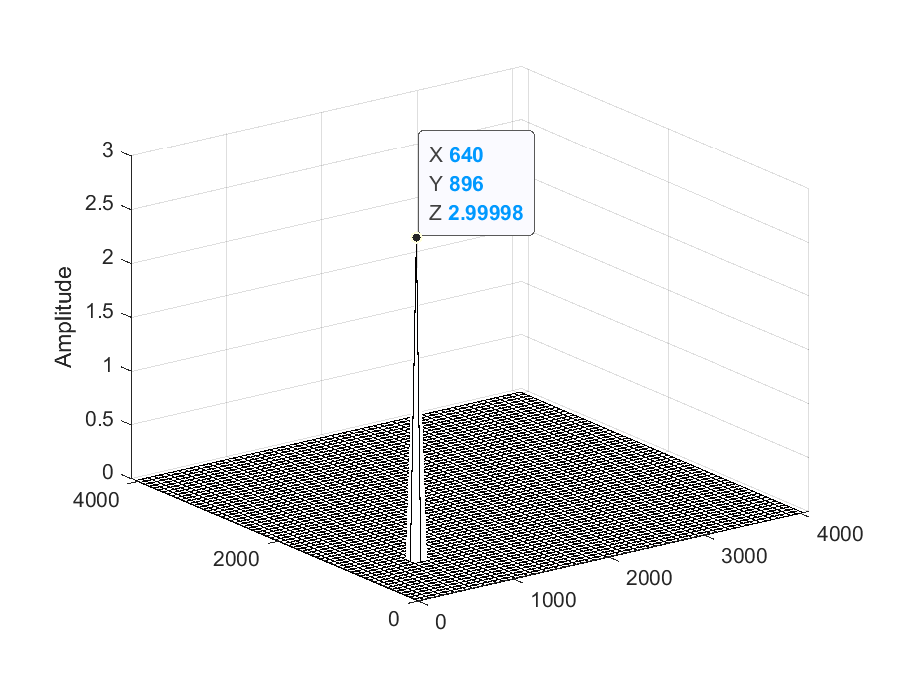
\includegraphics[width=60 mm]{fig/chirp_amp.eps}}
		\end{minipage}
		\label{chirp detect}	}
	\subfigure[The top view of \ref{chirp detect}.] {%第2张子图
		\begin{minipage}[]{35 mm} 	
			\centerline{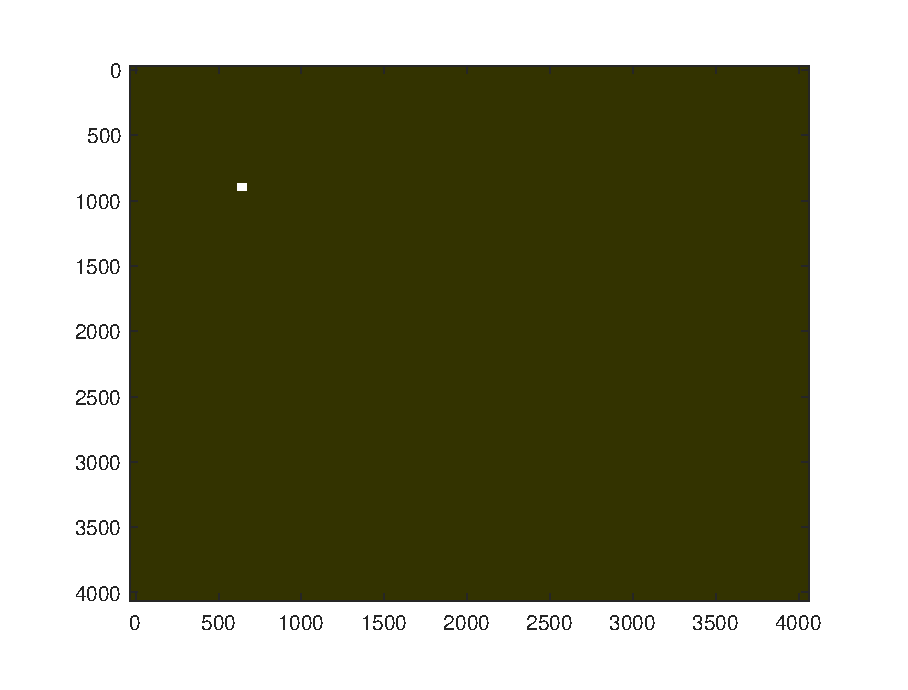
\includegraphics[width=45 mm]{fig/chirp_our.eps}}
		\end{minipage}
		\label{chirp detect overview}	}
	\caption{Chirp signal detection results.}  %大图名称	
	\label{chirp_our}
\end{figure}


\subsection{Fingerprint Feature Recognition}
%在这一小节,我们将考虑更复杂的信号,真实的指纹图像。一般的,指纹特征识别包含指纹的整体脊线流动模式、纹理构造的细节等.这是很耗时的分析过程。我们提出了分数傅里叶域的特征提取和识别,可以很快的获取指纹的主要特征。Gao提出,FRFT的相位具有相对时移不变性. 因此,我们提取的特征可以用于指纹的匹配。此外,指纹的纹理可以近似为多分量的2D chirp信号,因此在特定阶数下的分数阶傅里叶域是近似稀疏的。预处理后的指纹图像Fig5. 我们分别利用直接法和STDFRFT法实现了指纹的特征识别,如图所示。
In this subsection, we will consider more complex signals, real fingerprint images. Generally, fingerprint feature recognition includes the overall ridge flow pattern of the fingerprint, details of texture structure, etc. This is a time-consuming analysis process. We propose feature extraction and recognition in fractional Fourier domain, which can quickly obtain the main features of fingerprints. Gao\cite{b3} proposed that the phase of FRFT has relative time-shift invariance. Therefore, the extracted features in fractional Fourier domain can be used for fingerprint matching. Furthermore, the texture of the fingerprint can be approximated as a 2D chirp signal, and the fractional Fourier domain is almost sparse at a certain order. The preprocessed fingerprint signal is shown in {Fig. \ref{finger_origal}}. We use the direct method and the STDFRFT method to realize the feature recognition of fingerprints, as shown {in Fig. \ref{result by direct} and Fig. \ref{finger_STDFRFT}.} It is not difficult to find that our method can identify the main features of fingerprint signals in the fractional Fourier domain. And the effects of glitches and blurs are filtered out. {Furthermore, we simulate the incomplete fingerprint signal as shown in Fig. \ref{finger_loss}. The fingerprint features are identified by the STDFRFT method, and the result is displayed in Fig. \ref{finger_STDFRFT_loss}. By comparing with Fig. \ref{finger_STDFRFT}, we can know that our algorithm can extract the main features even for incomplete fingerprints.}




\begin{figure}[t]
	\centering
	\subfigure[Fingerprint image.] 	{%第一张子图
		\begin{minipage}[]{42 mm} 				
			\centerline{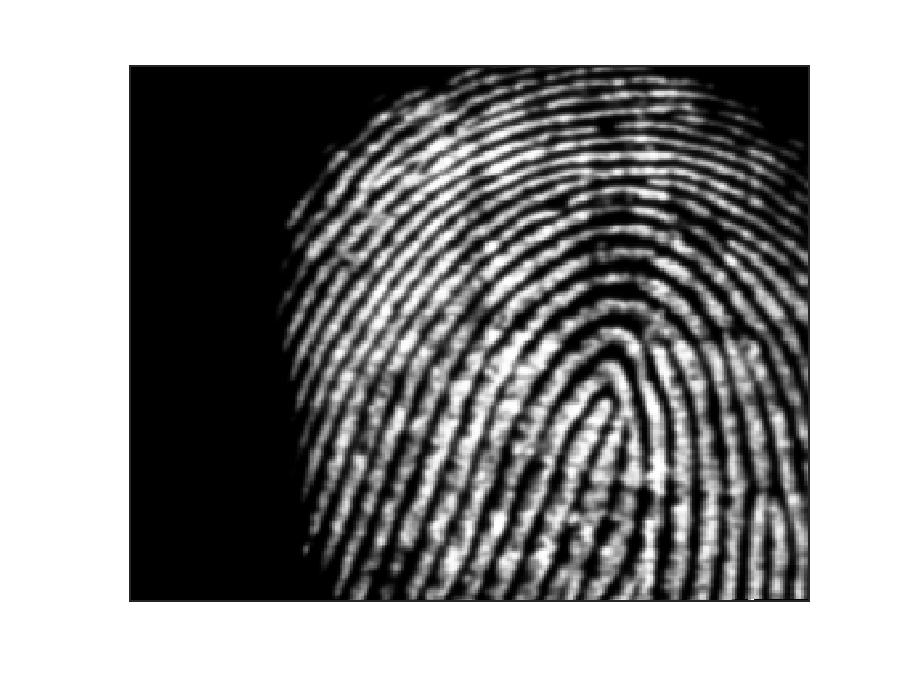
\includegraphics[width=50 mm]{fig/finger.eps}}
		\end{minipage}
		\label{finger_origal}	}
	\subfigure[{Incomplete fingerprint image.}] {%第2张子图
		\begin{minipage}[]{42 mm} 				
			\centerline{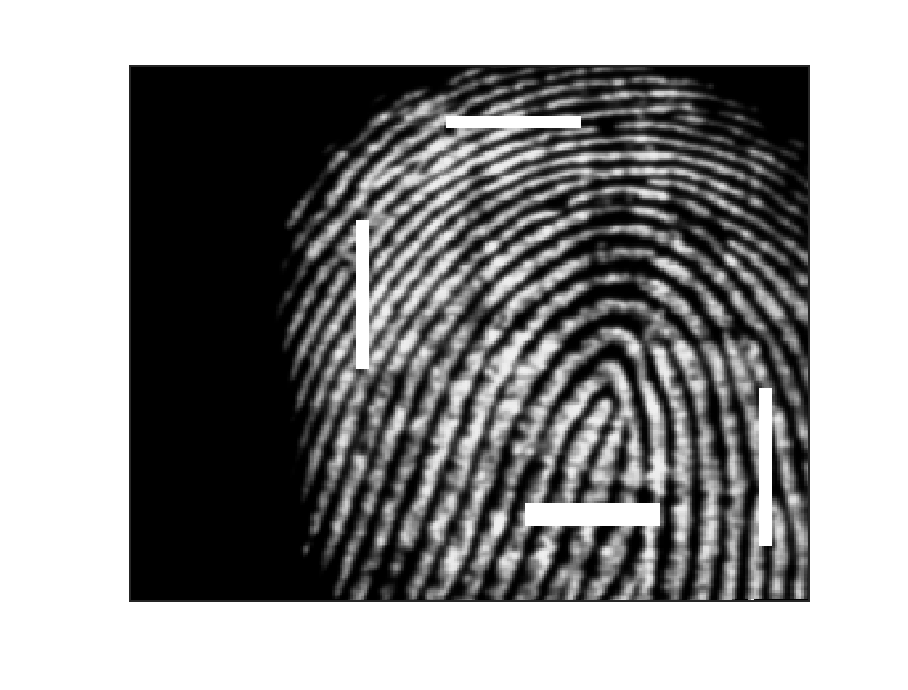
\includegraphics[width=50 mm]{fig/finger_loss.eps}}
		\end{minipage}
		\label{finger_loss}	}
	\caption{{Fingerprint images after preprocessing.}}  %大图名称	
	\label{finger}
\end{figure}

\begin{figure}[t]
	\centering
	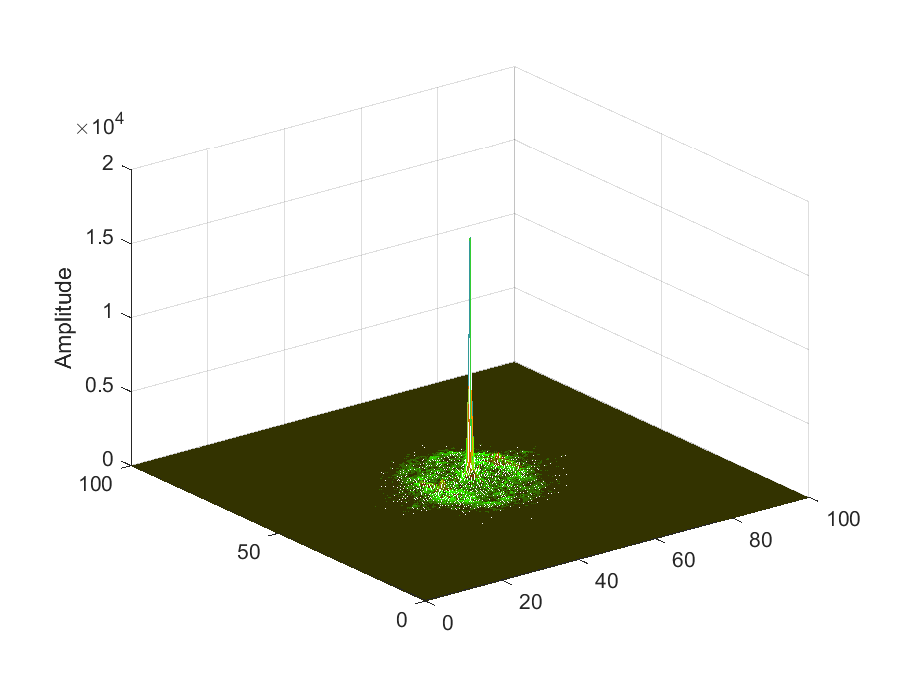
\includegraphics[width = 65 mm]{fig/finger_FRFD.eps}
	\caption{Recognition result of fingerprint in fractional domain by direct methed.}
	\label{result by direct} 
\end{figure}

\begin{figure}[t]	
	\subfigure[Our result for \ref{finger_origal}.] 	{%第一张子图
		\begin{minipage}[]{42 mm} 				
			\centerline{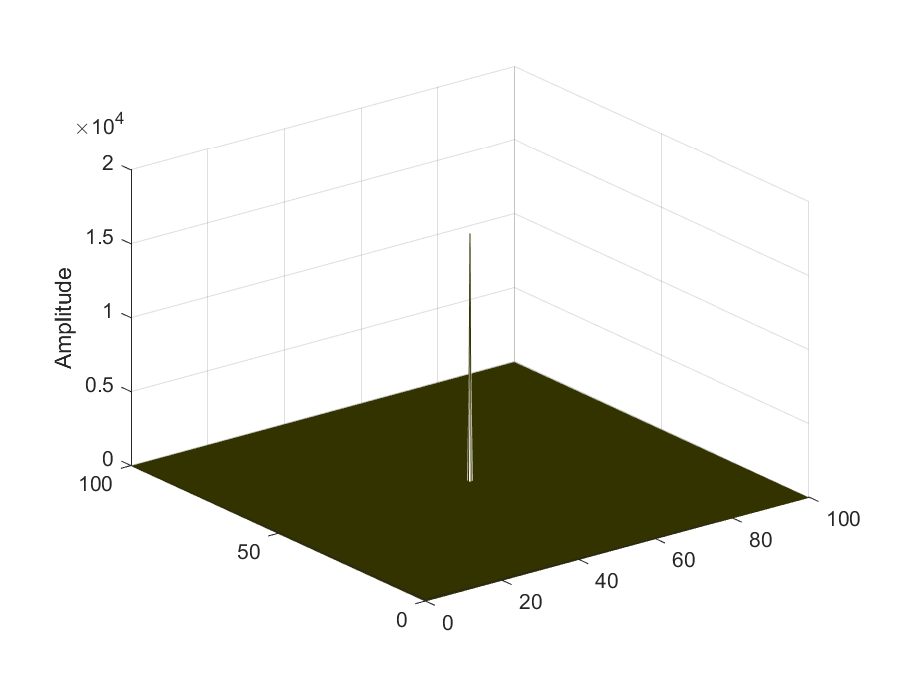
\includegraphics[width=50 mm]{fig/finger_STDFRFT.eps}}
		\end{minipage}
		\label{finger_STDFRFT}	}
	\subfigure[{Our result for \ref{finger_loss}.}] {%第2张子图
		\begin{minipage}[]{42 mm} 				
			\centerline{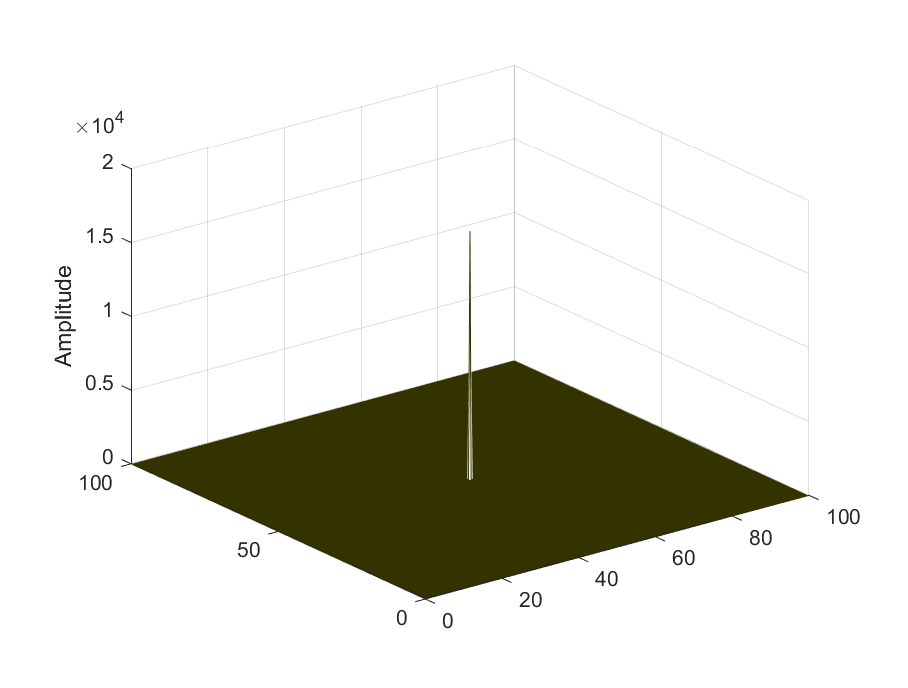
\includegraphics[width=50 mm]{fig/finger_STDFRFT_loss.eps}}
		\end{minipage}
		\label{finger_STDFRFT_loss}	}
	\caption{{Recognition result of fingerprints in fractional domain by our method.}}  %大图名称	
	\label{det_finger}
\end{figure}


%\begin{figure}[h]
%	\centering
%	\subfigure[Direct methed.] 	{%第一张子图
%		\begin{minipage}[]{65 mm} 				
%			\centerline{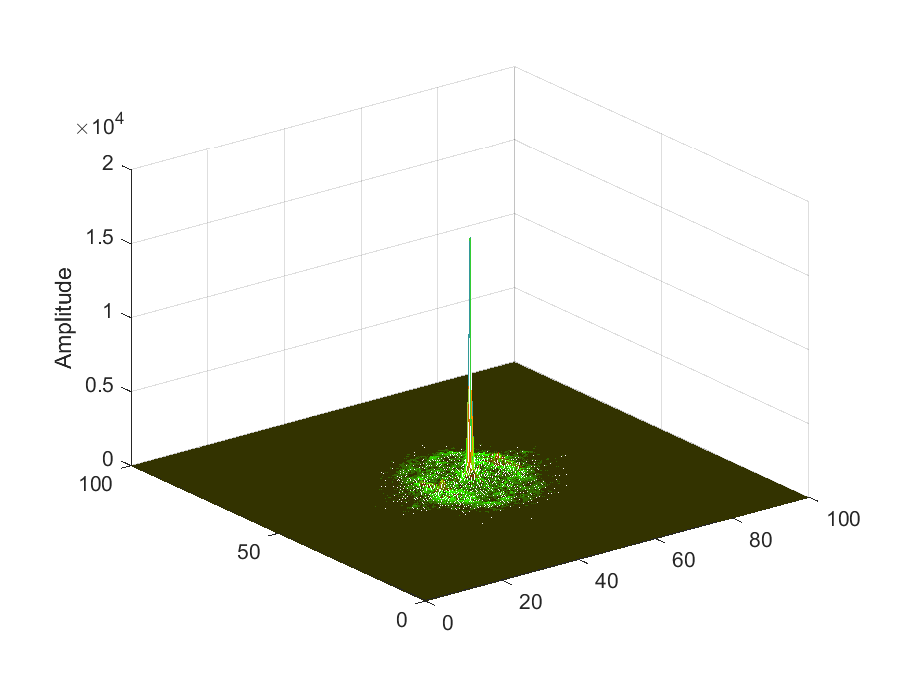
\includegraphics[width=65 mm]{fig/finger_FRFD.eps}}
%		\end{minipage}
%		\label{Decomp_finger}	}
%	\subfigure[Our methed.] {%第2张子图
%		\begin{minipage}[]{65 mm} 				
%			\centerline{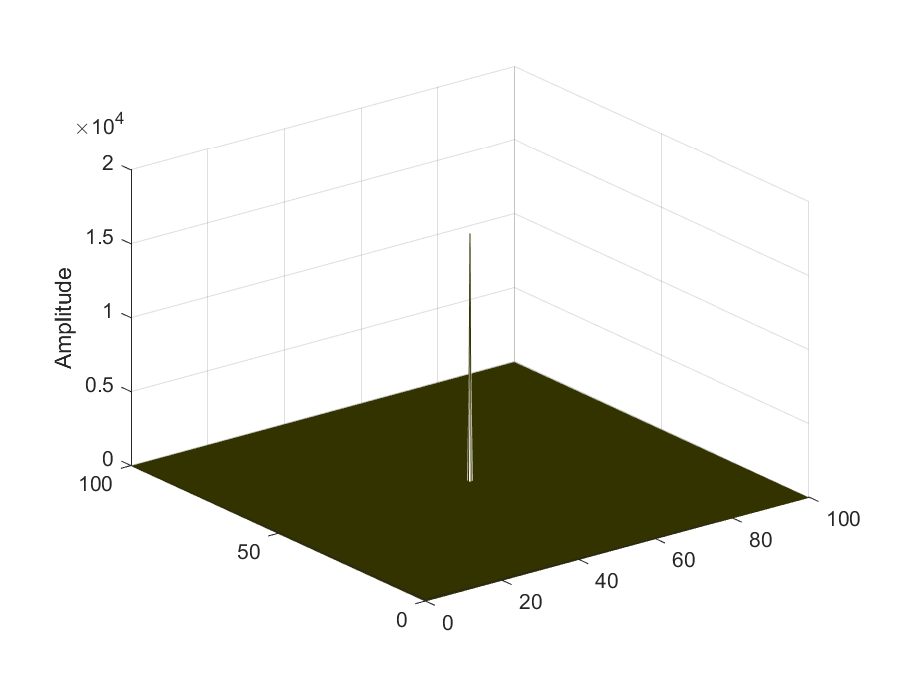
\includegraphics[width=65 mm]{fig/finger_STDFRFT.eps}}
%		\end{minipage}
%		\label{Our_finger}	}
%	\caption{Recognition Results of Finger in Fractional Domain.}  %大图名称	
%\label{det_finger}
%\end{figure}


%\subsection{Units}
%\begin{itemize}
%\item Use either SI (MKS) or CGS as primary units. (SI units are encouraged.) English units may be used as secondary units (in parentheses). An exception would be the use of English units as identifiers in trade, such as ``3.5-inch disk drive''.
%\item Avoid combining SI and CGS units, such as current in amperes and magnetic field in oersteds. This often leads to confusion because equations do not balance dimensionally. If you must use mixed units, clearly state the units for each quantity that you use in an equation.
%\item Do not mix complete spellings and abbreviations of units: ``Wb/m\textsuperscript{2}'' or ``webers per square meter'', not ``webers/m\textsuperscript{2}''. Spell out units when they appear in text: ``. . . a few henries'', not ``. . . a few H''.
%\item Use a zero before decimal points: ``0.25'', not ``.25''. Use ``cm\textsuperscript{3}'', not ``cc''.)
%\end{itemize}

%\subsection{Equations}

%\subsection{\LaTeX-Specific Advice}

%Please use ``soft'' (e.g., \verb|\eqref{Eq}|) cross references instead of ``hard'' references (e.g., \verb|(1)|). That will make it possible to combine sections, add equations, or change the order of figures or citations without having to go through the file line by line.
%Please don't use the \verb|{eqnarray}| equation environment. Use \verb|{align}| or \verb|{IEEEeqnarray}| instead. The \verb|{eqnarray}| environment leaves unsightly spaces around relation symbols.
%Please note that the \verb|{subequations}| environment in {\LaTeX} will increment the main equation counter even when there are no equation numbers displayed. If you forget that, you might write an article in which the equation numbers skip from (17) to (20), causing the copy editors to wonder if you've discovered a new method of counting.
%{\BibTeX} does not work by magic. It doesn't get the bibliographic data from thin air but from .bib files. If you use {\BibTeX} to produce a bibliography you must send the .bib files. 
%{\LaTeX} can't read your mind. If you assign the same label to a subsubsection and a table, you might find that Table I has been cross referenced as Table IV-B3. 
%{\LaTeX} does not have precognitive abilities. If you put a \verb|\label| command before the command that updates the counter it's supposed to be using, the label will pick up the last counter to be cross referenced instead. In particular, a \verb|\label| command should not go before the caption of a figure or a table.
%Do not use \verb|\nonumber| inside the \verb|{array}| environment. It will not stop equation numbers inside \verb|{array}| (there won't be any anyway) and it might stop a wanted equation number in the surrounding equation.

%\subsection{Some Common Mistakes}\label{SCM}
%\begin{itemize}
%\item The word ``data'' is plural, not singular.
%\item The subscript for the permeability of vacuum $\mu_{0}$, and other common scientific constants, is zero with subscript formatting, not a lowercase letter ``o''.
%\item In American English, commas, semicolons, periods, question and exclamation marks are located within quotation marks only when a complete thought or name is cited, such as a title or full quotation. When quotation marks are used, instead of a bold or italic typeface, to highlight a word or phrase, punctuation should appear outside of the quotation marks. A parenthetical phrase or statement at the end of a sentence is punctuated outside of the closing parenthesis (like this). (A parenthetical sentence is punctuated within the parentheses.)
%\item A graph within a graph is an ``inset'', not an ``insert''. The word alternatively is preferred to the word ``alternately'' (unless you really mean something that alternates).
%\item Do not use the word ``essentially'' to mean ``approximately'' or ``effectively''.
%\item In your paper title, if the words ``that uses'' can accurately replace the word ``using'', capitalize the ``u''; if not, keep using lower-cased.
%\item Be aware of the different meanings of the homophones ``affect'' and ``effect'', ``complement'' and ``compliment'', ``discreet'' and ``discrete'', ``principal'' and ``principle''.
%\item Do not confuse ``imply'' and ``infer''.
%\item The prefix ``non'' is not a word; it should be joined to the word it modifies, usually without a hyphen.
%\item There is no period after the ``et'' in the Latin abbreviation ``et al.''.
%\item The abbreviation ``i.e.'' means ``that is'', and the abbreviation ``e.g.'' means ``for example''.
%\end{itemize}
%An excellent style manual for science writers is \cite{b7}.

%\subsection{Identify the Headings}
%Headings, or heads, are organizational devices that guide the reader through your paper. There are two types: component heads and text heads.

%Component heads identify the different components of your paper and are not topically subordinate to each other. Examples include Acknowledgments and References and, for these, the correct style to use is ``Heading 5''. Use ``figure caption'' for your Figure captions, and ``table head'' for your table title. Run-in heads, such as ``Abstract'', will require you to apply a style (in this case, italic) in addition to the style provided by the drop down menu to differentiate the head from the text.

%Text heads organize the topics on a relational, hierarchical basis. For example, the paper title is the primary text head because all subsequent material relates and elaborates on this one topic. If there are two or more sub-topics, the next level head (uppercase Roman numerals) should be used and, conversely, if there are not at least two sub-topics, then no subheads should be introduced.

%\subsection{Figures and Tables}
%\paragraph{Positioning Figures and Tables} Place figures and tables at the top and bottom of columns. Avoid placing them in the middle of columns. Large figures and tables may span across both columns. Figure captions should be below the figures; table heads should appear above the tables. Insert figures and tables after they are cited in the text. Use the abbreviation ``Fig.~\ref{fig}'', even at the beginning of a sentence.

%\begin{table}[htbp]
%\caption{Table Type Styles}
%\begin{center}
%\begin{tabular}{|c|c|c|c|}
%\hline
%\textbf{Table}&\multicolumn{3}{|c|}{\textbf{Table Column Head}} \\
%\cline{2-4} 
%\textbf{Head} & \textbf{\textit{Table column subhead}}& \textbf{\textit{Subhead}}& \textbf{\textit{Subhead}} \\
%\hline
%copy& More table copy$^{\mathrm{a}}$& &  \\
%\hline
%\multicolumn{4}{l}{$^{\mathrm{a}}$Sample of a Table footnote.}
%\end{tabular}
%\label{tab1}
%\end{center}
%\end{table}

%\begin{figure}[htbp]
%\centerline{\includegraphics{fig1.png}}
%\caption{Example of a figure caption.}
%\label{fig}
%\end{figure}

%Figure Labels: Use 8 point Times New Roman for Figure labels. Use words rather than symbols or abbreviations when writing Figure axis labels to avoid confusing the reader. As an example, write the quantity ``Magnetization'', or ``Magnetization, M'', not just ``M''. If including units in the label, present them within parentheses. Do not label axes only with units. In the example, write ``Magnetization (A/m)'' or ``Magnetization \{A[m(1)]\}'', not just ``A/m''. Do not label axes with a ratio of quantities and units. For example, write ``Temperature (K)'', not ``Temperature/K''.

\section{Conclusions}
%在本文中,一个精确有效的2D FRFT快速算法被提出。相比于传统方法,提出的STDFRFT 在运行时间、L2误差、样本储存方面均表现更优。算法也成功地应用到了指纹的分数傅里叶域特征的识别。
In this paper, an accurate and efficient fast algorithm for 2D FRFT is proposed. Compared with the traditional method, the proposed STDFRFT performs better in terms of running time, $L_2$ error, and sample storage. Based on the fact that the fingerprint image can be approximated as 2D chirp signals, the algorithm is also successfully applied to the recognition of fractional Fourier domain features of fingerprints.
%The preferred spelling of the word ``acknowledgment'' in America is without an ``e'' after the ``g''. Avoid the stilted expression ``one of us (R. B. G.) thanks $\ldots$''. Instead, try ``R. B. G. thanks$\ldots$''. Put sponsor acknowledgments in the unnumbered footnote on the first page.

%\section*{References}
%Please number citations consecutively within brackets \cite{b1}. The sentence punctuation follows the bracket \cite{b2}. Refer simply to the reference number, as in \cite{b3}---do not use ``Ref. \cite{b3}'' or ``reference \cite{b3}'' except at the beginning of a sentence: ``Reference \cite{b3} was the first $\ldots$''
%Number footnotes separately in superscripts. Place the actual footnote at the bottom of the column in which it was cited. Do not put footnotes in the abstract or reference list. Use letters for table footnotes.

%Unless there are six authors or more give all authors' names; do not use ``et al.''. Papers that have not been published, even if they have been submitted for publication, should be cited as ``unpublished'' \cite{b4}. Papers that have been accepted for publication should be cited as ``in press'' \cite{b5}. Capitalize only the first word in a paper title, except for proper nouns and element symbols.

%For papers published in translation journals, please give the English citation first, followed by the original foreign-language citation \cite{b6}.

\bibliographystyle{IEEEtran}
\bibliography{IEEEabrv,refer}

%\begin{thebibliography}{00}
%\bibitem{b9} Bleay S M, Croxton R S, De Puit M. Fingerprint development techniques: theory and application[M]. 2018.
%\bibitem{Sun2022} {Sun L, Wang X, Huang Z, et al. Radio frequency fingerprint extraction based on feature inhomogeneity[J]. IEEE Internet of Things Journal, 2022.}
%\bibitem{Mehboob2022} {Mehboob R, Dawood H. DEHFF–A hybrid approach based on distinctively encoded fingerprint features for live fingerprint detection[J]. Biomedical Signal Processing and Control, 2022, 75: 103572.}
%\bibitem{Kumar2022} {Kumar T, Bhushan S, Jangra S. Ann trained and WOA optimized feature-level fusion of iris and fingerprint[J]. Materials Today: Proceedings, 2022, 51: 1-11.}
%%\bibitem{b7} Roddy A R, Stosz J D. Fingerprint features-statistical analysis and system performance estimates. Proceedings of the IEEE, 1997, 85(9): 1390-1421.
%%\bibitem{b10} Jain A K, Chen Y, Demirkus M. Pores and ridges: High-resolution fingerprint matching using level 3 features. IEEE transactions on pattern analysis and machine intelligence, 2006, 29(1): 15-27.
%%\bibitem{b8} Cao K, Yang X, Chen X, et al. Minutia handedness: A novel global feature for minutiae-based fingerprint matching. Pattern recognition letters, 2012, 33(10): 1411-1421.
%\bibitem{b6} Sejdić E, Djurović I, Stanković L J. Fractional Fourier transform as a signal processing tool: An overview of recent developments. Signal Processing, 2011, 91(6): 1351-1369.
%\bibitem{b4} Su X, Tao R, Kang X. Analysis and comparison of discrete fractional Fourier transforms. Signal Processing, 2019, 160: 284-298.
%
%\bibitem{b2} Pei S C, Ding J J. Closed-form discrete fractional and affine Fourier transforms. IEEE Transactions on Signal Processing, 2000, 48(5): 1338-1353. 
%\bibitem{Kumari2021} {Kumari R, Mustafi A. An optimized framework for digital watermarking based on multi-parameterized 2D-FrFT using PSO[J]. Optik, 2021, 248: 168077.}
%
%%\bibitem{b5} Saxena N, Sharma K K. Pansharpening scheme using filtering in two-dimensional discrete fractional Fourier transform. IET Image Processing, 2018, 12(6): 1013-1019.
%
%\bibitem{b1} Wang S, Patel V M, Petropulu A. Multidimensional sparse Fourier transform based on the Fourier projection-slice theorem. IEEE Transactions on Signal Processing, 2018, 67(1): 54-69.
%\bibitem{Ozaktas} {Ozaktas H M, Arikan O, Kutay M A, et al. Digital computation of the fractional Fourier transform[J]. IEEE Transactions on signal processing, 1996, 44(9): 2141-2150.}
%\bibitem{JR} {José R, Juliano B, Gilson J, et al. Computation of an eigendecomposition-based discrete fractional Fourier transform with reduced arithmetic complexity[J]. Signal Processing, 2019, 165: 72-82.}
%\bibitem{b3} Gao L, Qi L, Guan L. The spatial shift operations on image reconstruction from 2D-FRFT information with application to SAR moving target detection//2013 IEEE China Summit and International Conference on Signal and Information Processing. IEEE, 2013: 523-527.
%
%\end{thebibliography}
%\vspace{12pt}
%\color{red}
%IEEE conference templates contain guidance text for composing and formatting conference papers. Please ensure that all template text is removed from your conference paper prior to submission to the conference. Failure to remove the template text from your paper may result in your paper not being published.

\end{document}
